\section{Trajectory Generation}\label{sec:trajectory_generation}\todo{Wyatt, any references for trajectory generation stuff that would be useful for this section?}

Another major compenent of the path execution subsystem developed in this thesis is trajectory generation. This componenet sits between the steering and path planning components, taking global paths from path planning and outputting desired states that the steering component attempts to achieve. The trajectory generator fills the same role as the ``base\_local\_planner'' described in \autoref{subsec:base_local_planner}. The input to the trajectory generator is an ordered sequence of path segments (called a \emph{path}). The path segments are described in \autoref{subsec:path_segment}. The output is a desired state for the current timestep, as described in \autoref{subsec:steering_state}.

\subsection{Path Segment Description}\label{subsec:path_segment}

The path segment used by the trajectory generator developed for this thesis is described in \autoref{table:path_segment_description}. There are three different types of path segments used in this thesis -- straight lines, smooth constant curvature arcs and spin-in-places. One important assumption about these path segments is that, for a given sequence of segments, they will already be bleneded together to remove any discontinuities in the geometric parameterization between the end of a segment and the beginning of the following segment.

\begin{table}[htbp]
	\begin{tabularx}{\textwidth}{|r|X|}
		\hline
		Name & Description \\
		\hline
		header & This is a standard ROS header type that contains information such as the reference frame the rest of the fields are in and the timestamp for when the path segment was generated \\
		\hline
		segment\_type & An integer enum representing the type this segment, such as a straight line segment, constant curvature arc segment or spin-in-place segment. \\
		\hline
		segment\_number & The ID number of the segment that generated this state. \\
		\hline
		segment\_length & The length of the segment. Whether it is in meters or radians depends on the \emph{segment\_type} \\
		\hline
		reference\_point & The reference point for this path segment. Interpretation depends on the \emph{segment\_type} \\
		\hline
		initial\_tangent\_angle & The intial tangent angle for this segment. Interpretation depends on the \emph{segment\_type} \\
		\hline
		curvature & The curvature of this segment. Exact interpretation depends on the \emph{segment\_type}. For straight lines curvature should be 0.0 \\
		\hline
		max\_speed & A pair of the maximum translational speed and maximum rotational speed to be used for this segment \\
		\hline
		min\_speed & A pair of the minimum translational speed and minimum rotational speed to be used for this segment \\	
		\hline
		acceleration\_limit & The acceleration limit for this segment. Whether it is in $m/s^2$ or $rads/s^2$ depends on the \emph{segment\_type} \\
		\hline
		deceleration\_limit	& The deceleration limit for this segment. Whether it is in $m/s^2$ or $rads/s^2$ depends on the \emph{segment\_type} \\
		\hline
	\end{tabularx}
	\caption{Path Segment State Field Description \label{table:path_segment_description}}
\end{table}

Of the fields listed in \autoref{table:path_segment_description}, the ones requiring the most explanation are the \emph{reference\_point} and the \emph{initial\_tangent\_angle}. The \emph{reference\_point} can have the following meanings, depending on \emph{segment\_type}. For a straight line segment, the reference point is the start point of the line segment. For a constant curvature arc, the reference point is the center of the circle that the arc belongs to (the radius of that circle is $1/curvature$). For a spin-in-place segment, the reference point is the point about which to spin. The \emph{initial\_tangent\_angle} can have the following means, depending on \emph{segment\_type}. For a straight line segment, the initial tangent angle is the direction of the line segment. For a constant curvature arc, the initial tangent angle defines the actual point along the circle where the the arc segment begins. For a spin-in-place segment, the initial tangent angle is angle that the spin should start from.

As discussed in \autoref{subsec:steering_state}, the spin-in-place segment type was added to the original path segment types to avoid numerical instability issues when using arcs with very small radii.

\subsection{Trajectory Generation Algorithm}\label{subsec:trajectory_generation_algorithm}

The trajectory generation algorithm used in this thesis is detailed in this section. On HARLIE, this loop ran at 20 Hz to regularly send commands to the steering algorithms detailed in \autoref{subsec:steering_algorithms}. Note that the trajectory generator and steering algorithm, while both run at 20 Hz, they are not explicitly synchronized. It should also be noted that, while many of these concepts are not limited to SE(2) space (position and rotation on the XY plane), these algoritms are written assuming SE(2) space and not a more generalized six degree of freedom system (SE(3) space). \todo{add some references about SE(2) and SE(3) space}

\todo{Better access to the struct things when they are like $state_t.velocity$}
\todo{Use $\leftarrow$ or = for assignment of variables in algorithms?}
\todo{add figure of the different path segments with labels for the geometric primitive bits and the desired state output}

\begin{algorithm}
\caption{Trajectory Generation Algorithm}
\label{alg:trajectory_generation_algorithm}
\DontPrintSemicolon
\SetKwFunction{MakeHaltState}{MakeHaltState}
\SetKwFunction{GetCurrentRobotState}{GetCurrentRobotState}
\SetKwFunction{UpdateSegmentNumberAndDistance}{UpdateSegNumAndDist}
\SetKwFunction{ComputeVelocityCommand}{ComputeVelocityCommand}
\SetKwFunction{ComputeDesiredPose}{ComputeDesiredPose}

\KwIn{$state_{t-1}$, $path$, $i_{t-1}$, $l_{t-1}$}
\KwOut{$state_t$, $i_t$, $l_t$}

$robot\_state_t$ = \GetCurrentRobotState{} \;
\eIf{path $\neq \emptyset$}
{
	\tcp{Compute new desired state}
	$i_t$, $l_t$ = \UpdateSegmentNumberAndDistance{$robot\_state_t$, $path$, $i_{t-1}$, $l_{t-1}$, $state_{t-1}$} \;
	$v_t$ = \ComputeVelocityCommand{$path$, $i_t$, $l_t$} \;
	$pose_t$ = \ComputeDesiredPose{$path$, $i_t$, $l_t$} \;
	$state_t.segment\_type$ = $path\left[i_t\right].segment\_type$ \;
	$state_t.pose$ = $pose_t$ \;
	$state_t.rho$ = $path\left[i_t\right].curvature$ \;
	$state_t.velocity$ = $v_t$ \;
	\;
	\tcp{Check new desired state for collisions}
	\If{$state_t$ will be in collision}
	{
		$state_t$ = \MakeHaltState{$robot\_state_t$} \;
	}
}
{
	$i_t$ = $0$ \;
	$l_t$ = $0.0$ \;
	$state_t$ = \MakeHaltState{$robot\_state_t$} \;
}
\end{algorithm}

\autoref{alg:trajectory_generation_algorithm} describes the trajectory generation algorithm that runs at the loop rate of 20 Hz. Its inputs are the last desired state ($state_{t-1}$), the current path from the path planner ($path$), the last segment number being executed ($i_{t-1}$) and the distance traveled along that segment already ($l_{t-1}$). The outputs (which are fed into the the algorithm on the next loop as well as being sent to the steering algorithm) are the current desired state ($state_t$), the current segment number being executed ($i_t$) and the distance traveled along that segment after this loop ends ($l_t$). Note that the segment number being executed, $i_t$, is an index into the sequence of path segments contained in the $path$. Also note that all of the algorithms described here assume that positions and orientations have all been placed in the same reference frame; on HARLIE, this was done with the ROS ``tf'' library (see \todo{add ref to ros tf library}).

There are a number of algorithms used in \autoref{alg:trajectory_generation_algorithm}. Two of these are fairly simple: \GetCurrentRobotState and \MakeHaltState. \GetCurrentRobotState gets the current robot position, orientation and velocities in a robot specific manner. For HARLIE, this information came from the output of the localization subsystem described in \autoref{sec:localization}. \MakeHaltState takes the give state (usually the current robot state) and generates a state that would cause the steering algorithms to stop and maintain that state. In this case, it simply generates a spin-in-place state at the robot's current position and orientation with zero speeds and curvatures; effectively, this state causes steering to stop both translational and rotational motion until given a new commanded state.

\SetKwFunction{Length}{Length}

The other three algorithms used in \autoref{alg:trajectory_generation_algorithm} are more complicated and require more detailed explanation. In all of these algortihms, \Length is a simple function that returns the number of path segments in the $path$ it is given. These algorithms are based on zero-indexed sequences (such as arrays in C) as opposed to one-indexed containers such as those found in Matlab. Also, in all of these algorithms, $dt$ is the time since the last loop ended (on HARLIE, $dt = \frac{1}{20 Hz}$).

\begin{algorithm}
\caption{Update Segment Number and Distance Algorithm}
\label{alg:update_seg_num_and_dist_algorithm}
\DontPrintSemicolon

\KwIn{$robot\_state_t$, $path$, $i_{t-1}$, $l_{t-1}$, $state_{t-1}$}
\KwOut{$i_t$, $l_t$}

\If{$i_{t-1} \geq \Length{path}$}
{
	$i_t$ = $\Length{path}-1$ \;
	$end$ = true \;
}

$\delta l$ = $state_{t-1}.velocity \cdot dt$ \;

\eIf{$path\left[i_t\right]$ is a spin-in-place segment}
{
	$l_t$ = $l_{t-1} + \delta l$ \;	
}
{
	$l_t$ = $l_{t-1} + \delta l \cdot \cos\left(state_{t-1}.orientation - robot\_state_t.orientation\right) $ \; \nllabel{update_seg_num_project_onto_des_tangent_vec}
}

$\hat l$ = $path\left[i_t\right].segment\_length$ \;
\If{$l_t > \hat l$}
{
	$l_t$ = $0.0$ \;
	$i_t$ = $i_t + 1$ \;
}

\If{$i_t \geq \Length{path}$}
{
	$i_t$ = $\Length{path}-1$ \;
	$end$ = true \;
}

$\hat l$ = $path\left[i_t\right].segment\_length$ \; \nllabel{update_seg_num_seg_num_may_have_changed}

\If{$end$ is true}
{
	$l_t$ = $\hat l$ \;
}

\end{algorithm}

\autoref{alg:update_seg_num_and_dist_algorithm} is the \UpdateSegmentNumberAndDistance function used in \autoref{alg:trajectory_generation_algorithm}. Its inputs are the current robot state ($robot\_state_t$), the current path ($path$), the last segment number being executed ($i_{t-1}$), the distance traveled along that segment already ($l_{t-1}$) and the last desired state ($state_{t-1}$). \autoref{alg:update_seg_num_and_dist_algorithm} then updates the distance traveled along the current segment according to the velocity in $state_{t-1}$ while moving to the next segment when appropriate and not running past the end of the $path$. It then outputs these new values for the segment number being executed ($i_t$) and distance already traveled along that segment ($l_t$) for consumption by the remainder of \autoref{alg:trajectory_generation_algorithm}.

Two important details of this computation are on \autoref{update_seg_num_project_onto_des_tangent_vec} and \autoref{update_seg_num_seg_num_may_have_changed} of \autoref{alg:update_seg_num_and_dist_algorithm}. \autoref{update_seg_num_project_onto_des_tangent_vec} projects the robot's motion onto the the tangent vector of the last state. This prevents situations where the robot is moving nearly orthogonal to the desired state's tangent vector from advancing the distance traveled along the path segment too far for the actual distance along the path segment traveled. These situations can occur while using \emph{phase space steering} if there is a large lateral offset from the path -- \emph{phase space steering} is designed to move nearly orthogonal to the desired state's tangent vector in that situation. \autoref{update_seg_num_seg_num_may_have_changed} is required to ensure that the correct segment current segment and segment length is selected, even after all of the adjustments to the current segment number ($i_t$) have been made.

\begin{algorithm}
\caption{Compute Velocity Command Algorithm}
\label{alg:compute_velocity_command_algorithm}
\DontPrintSemicolon

\KwIn{$path$, $i_t$, $l_t$}
\KwOut{$v_t$}

\eIf{$path\left[i_t\right]$ is a spin-in-place segment}
{
	$v_{t+1}$ = $0.0$ \;
	$v_t$ = $path\left[i_t\right].max\_speed.omega$ \;
}
{
	$v_t$ = $path\left[i_t\right].max\_speed.linear$ \;
	\eIf{$i_t < \Length{path} - 1$}
	{
		$v_{t+1}$ = $path\left[i_t + 1 \right].max\_speed.linear$ \;
	}
	{
		$v_{t+1}$ = $0.0$ \;
	}
}

$dec$ = $path\left[i_t\right].deceleration\_limit$ \;
$dec\_dist$ = $\frac{\left( v_t + v_{t+1} \right)}{2.0} \cdot \frac{\left( v_t - v_{t+1} \right)}{dec}$ \;

$rem$ = $path\left[i_t\right].segment\_length - l_t$ \;
\uIf{$rem < 0.0$}
{
	$rem$ = $0.0$ \;
}
\uElseIf{$rem < dec\_dist$}
{
	$v_t$ = $\sqrt{2.0 \cdot rem \cdot dec + v_{t+1}^2}$ \;
}
\Else
{
	$v_t$ = $v_t + path\left[i_t\right].accel\_limit \cdot dt$ \;
}

\eIf{$path\left[i_t\right]$ is a spin-in-place segment}
{
	clamp $v_t$ to interval $\left[ path\left[i_t\right].min\_speed.omega, path\left[i_t\right].max\_speed.omega \right]$ \;
}
{
	clamp $v_t$ to interval $\left[ path\left[i_t\right].min\_speed.linear, path\left[i_t\right].max\_speed.linear \right]$ \;
}

\end{algorithm}

\autoref{alg:compute_velocity_command_algorithm} is the \ComputeVelocityCommand function used in \autoref{alg:trajectory_generation_algorithm}. Its inputs are the current path ($path$), the segment number being executed ($i_t$) and distance already traveled along that segment ($l_t$), as output by \autoref{alg:update_seg_num_and_dist_algorithm}. Its only output is the desired velocity command ($v_t$). \autoref{alg:compute_velocity_command_algorithm} has three steps. First, the algorithm initializes to the max speed for the current segment ($v_t$) and determines the max speed of the next segment ($v_{t+1}$). Next, it determines whether it can continue accelerating or needs to start braking in order to slow down to $v_{t+1}$ before the beginning of the next segment. Finally, the calculated velocity command $v_t$ is clamped to fall within the interval defined by the current segment's minimum and maximum speeds. After clamping, $v_t$ calculation is complete.

\begin{algorithm}
\caption{Compute Desired Pose Algorithm}
\label{alg:compute_desired_pose_algorithm}
\DontPrintSemicolon

\KwIn{$path$, $i_t$, $l_t$}
\KwOut{$pose_t$}

$\Psi$  = $path\left[i_t\right].init\_tan\_angle$ \;
\Switch{$path\left[i_t\right].segment_type$}
{
	\Case{straight line segment}
	{
		$pose_t.position$ = $path\left[i_t\right].reference\_point + l_t \cdot 
			\begin{bmatrix}
				\cos \Psi \\
				\sin \Psi \\
			\end{bmatrix} $ \;
		$pose_t.orientation$  = $\Psi$ \;
	}
	\Case{constant curvature arc segment}
	{
		$\rho$ = $path\left[i_t\right].curvature$ \;
		$r$ = $\frac{1}{ | \rho | }$ \;
		\eIf{$\rho \geq 0.0$}
		{
			$\hat\Psi$ = $\Psi - \frac{\pi}{2}$ \;
		}
		{
			$\hat\Psi$ = $\Psi + \frac{\pi}{2}$ \;
		}
		$\delta\Psi$ = $l_t \cdot \rho$ \;
		$pose_t.position$ = $path\left[i_t\right].reference\_point + r \cdot 
			\begin{bmatrix}
				\cos\left( \hat\Psi + \delta\Psi \right) \\
				\sin\left( \hat\Psi + \delta\Psi \right) \\
			\end{bmatrix} $ \;
		$pose_t.orientation$  = $\Psi + \delta\Psi$ \;
	}
	\Case{spin-in-place segment}
	{
		$\rho$ = $path\left[i_t\right].curvature$ \;
		\eIf{$\rho \geq 0.0$}
		{
			$\hat\Psi$ = $\Psi - \frac{\pi}{2}$ \;
		}
		{
			$\hat\Psi$ = $\Psi + \frac{\pi}{2}$ \;
		}
		$\delta\Psi$ = $l_t \cdot \rho$ \;
		$pose_t.position$ = $path\left[i_t\right].reference\_point$ \;
		$pose_t.orientation$  = $\Psi + \delta\Psi$ \;
	}
}

\end{algorithm}

\autoref{alg:compute_desired_pose_algorithm} is the \ComputeDesiredPose function used in \autoref{alg:trajectory_generation_algorithm}. Its inputs are the current path ($path$), the segment number being executed ($i_t$) and distance already traveled along that segment ($l_t$), as output by \autoref{alg:update_seg_num_and_dist_algorithm}. Its only output is the desired pose ($pose_t$). \autoref{alg:compute_desired_pose_algorithm} is made up of three cases, depending on what type of path segment the pose is being computed from. For a straight line segment, \autoref{alg:compute_desired_pose_algorithm} moves the reference point in the direction of the tangent vector (as defined by the path segment's initial tangent angle and sets the orientation to face along that tangent vector. For a constant curvature arc segment, it must find the correct point along the circle $\frac{1}{ | \rho | }$ away from the segment's reference point as well as compute the correct tangent angle for that point on the circle. For a spin-in-place segment, it only needs to set the desired pose's orientation according to how far along the segment the trajectory generator is; because it is a spin-in-place, the desired position is the same as the segment's reference point.

\subsection{Adding Feedback for Planning}\label{subsec:trajectory_generation_actionlib}

In the original design of the trajectory generator, the outputs of \autoref{alg:trajectory_generation_algorithm} were not exposed outside of the trajectory generation subsystem. Things like the current path ($path$), the segment number being executed ($i_t$) and distance already traveled along that segment ($l_t$) were only fed back into \autoref{alg:trajectory_generation_algorithm}. This lack of information became a problem for the path planning system when it needed to replan around a dynamic (or otherwise unexpected) obstacle that invalidated the original path plan. In order to replan efficiently, the path planner needed to be aware of where along the previous path plan the trajectory generator was when it encountered the obstacle. Without that information, the path planner was unable to generate a new path plan that avoided the obstacle and was still smoothly blended with the segments of the original plan that were unaffected by the obstacle's presence. To provide the path planner with the information required, the trajectory generator output the $path$ it was currently using, the current segment being executed $i_t$ and the distance traveled along that segment $l_t$. With this information, the path planner could easily extrapolate exactly where the trajectory generator had commanded the robot before detecting the collision and efficiently modify the path to avoid that collision. On HARLIE, this feedback mechanism was implemented using the ROS ``actionlib'' \todo{add ref to actionlib docs} library.

\subsection{Collision Detection}\label{subsec:trajectory_generation_costmap3d}

\begin{figure}
\centering
\subfloat[Side View, 20cm Resolution]{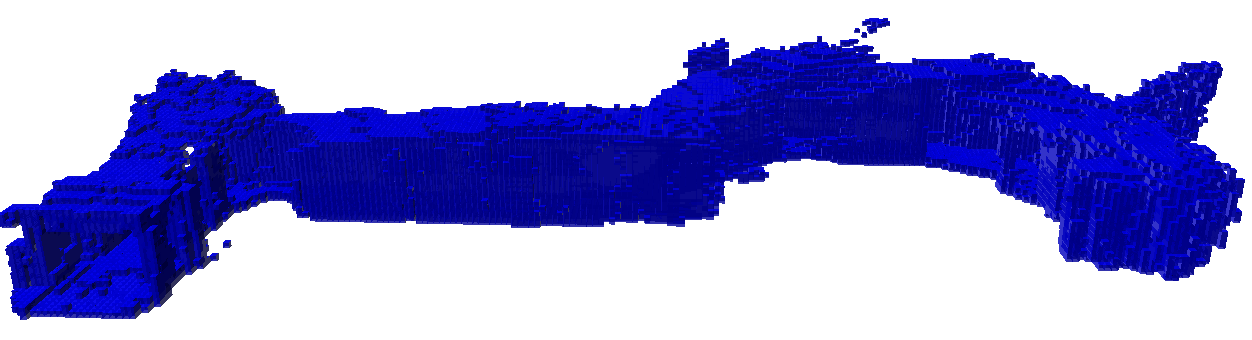
\includegraphics[width=0.75\textwidth]{images/3rd_floor_side_20cm}\label{fig:costmap3d_examples_side_view}}
\\
\subfloat[Inside View, 2.5cm Resolution]{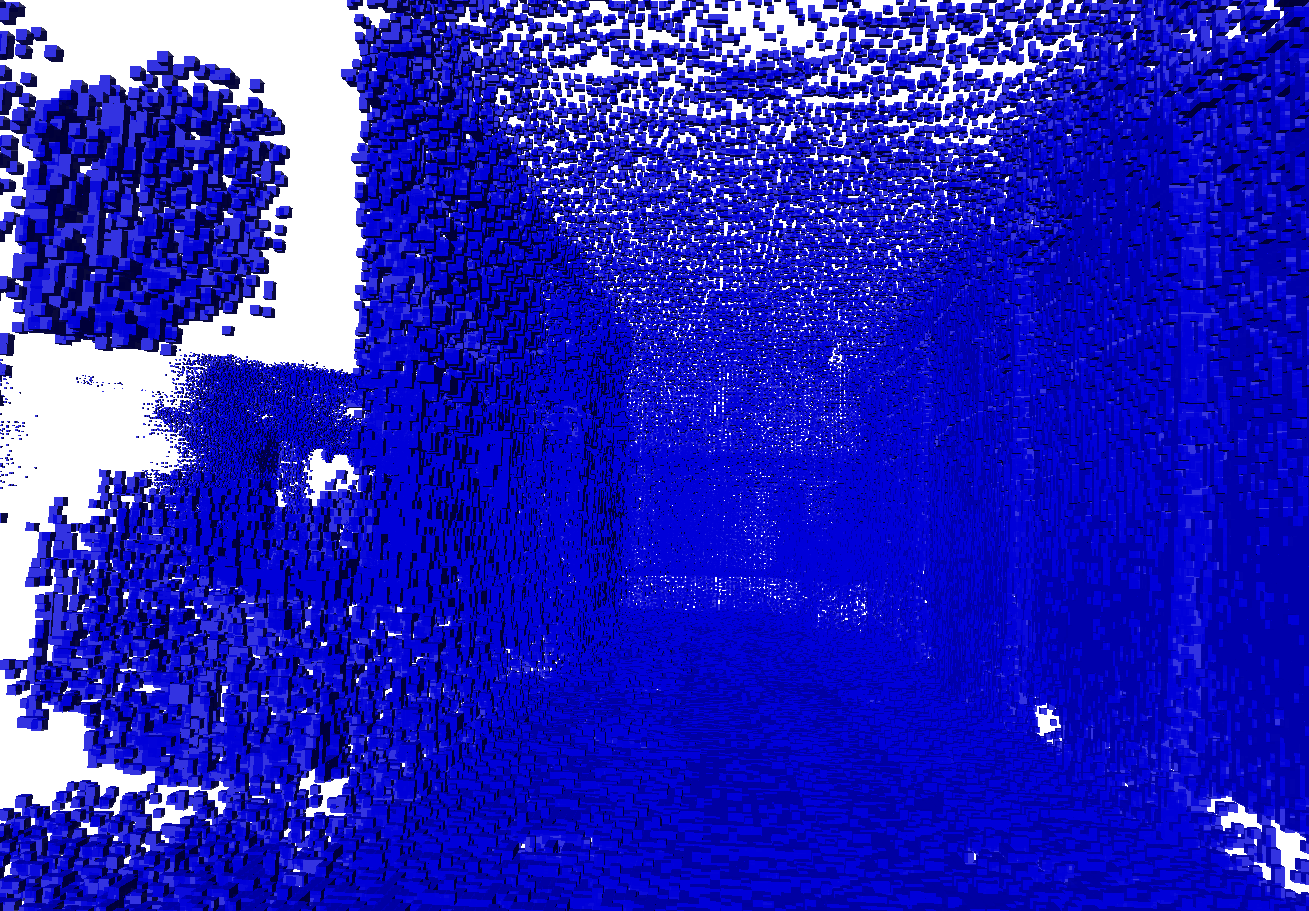
\includegraphics[width=0.75\textwidth]{images/3rd_floor_inside_2_5cm}\label{fig:costmap3d_examples_inside_view}}
\caption[Costmap3D Examples]{Costmap3D Examples. These are from an OctoMap built from 3D sensor data of the Glennan 3rd Floor while using Costmap3D.}
\label{fig:costmap3d_examples}
\end{figure}

In order to do precise navigation in complex, dynamic environments it is not simply enough to precisely follow a planned path -- the system must also avoid collisions with objects in the environment. The first step to avoid a collision is detecting that it is going to occur. There were two different methods for collision detection used in this trajectory generation subsystem: one based on existing ROS obstacle mapping and the other based on an octree representation of the environment. The original collision detection system used functionality based on the ROS ``costmap\_2d'' described in \autoref{subsec:costmap_2d}. This method suffered from many of the drawbacks described in \autoref{subsec:costmap_2d}, specifically the difficulty of maintaining a high resolution obstacle map in an efficient manner. The collision detection system itself was also difficult to use for checking the collision of a single pose efficiently; since the functionaltiy was originally part of the ROS ``base\_local\_planner'' (see \autoref{subsec:base_local_planner}), it was designed for checking a set of controls from the current robot pose and not a given state that was part of a path segment. It also did not have support for forward simulating, while checking for collisions, a desired state along one of the path segments used in this thesis, but could only forward simulate a set of constant velocity commands (translational and rotational).

To address these shortcomings in the existing ROS obstacle mapping, a new obstacle mapping component was developed for use by trajectory generation. This component, called ``costmap3d'' uses the OctoMap library \autocite{octomap} to allow efficient, hi-resolution 3D collision checking in large environments (see \autoref{fig:costmap3d_examples} for an example of an OctoMap created by ``costmap3d''). ``costmap3d'' improves three of the issues with the ROS obstacle mapping and collision checking mentioned above and in \autoref{subsec:costmap_2d}: simplistic integration of sensor measurements over time, efficiently representing large environments at small resolutions and a simple method for efficiently checking a single position in the map for collisions.

The first two issues, simplistic integration of sensor measuremnts over time and efficiently representing large environments at small resolutions, are addressed via the use of the OctoMap library. OctoMap uses a probabilistic representation of sensor measurements (derived from the occupancy grid mapping techniques introduced in \autocite{Moravec_1985_1840}) to compute the probability of a given map cell being either free space or occupied. This means that the occupancy state of a map cell is based on all of the previous measurements that intersected with that cell and not simply the last measurement that did so (as is the case in ``costmap\_2d'').

OctoMap also solves the issue of efficiently representing large environments at small resolutions. It does so by using an octree representation for the map as opposed to a fixed size grid (where the cells can either be 2D as in the case of ``costmap\_2d'' or 3D as in the case of a voxel grid). Octrees, very similar to quadtrees used for 2D environments, are a nested, recursive datastructure where each voxel in the octree can be further subdivided into eight more voxels, thereby forming an octree inside of that voxel (see \todo{add Octree figure from octomap paper for visualizing how an Octree structure looks} \todo{add reference to something describing octrees}). Because groups of smaller voxels with the same label can be represented by keeping the containing larger voxel, octrees can represent very large environments at high resolutions with little memory usage (compared to a traditional fixed size occupancy grid). For example, an empty hallway with a door at the end, a common environment for this precision navigation system, can easily be represented by an octree by maintaing the large, parent voxels in the empty hallway while using small voxels to represent the area near the doorway at a small enough resolution such that the doorway does not occlude free space simply because the grid size is too large. To do this, OctoMap regularly ``prunes'' the underlying octree occupancy map to merge groups of voxels that have the same occupancy label (e.g. free or obstalce) into a single, larger containing parent voxel with that same label. After pruning, there is no need to keep the children in memory as they are losslessly represented by the parent voxel; this greatly reduces the memory requirements for representing large environments at high resolution, especially if those environments can be grouped into clumps of free and occupied space.

Though OctoMap solves the obstacle mapping issues of ``costmap\_2d'' described above, the OctoMap library itself does not have any facilities for efficiently checking a given robot pose for collisions. OctoMap does provide functionality for getting the occupancy state of a given point, but no facilities for checking something like the bounding box of the robot at a given pose. That is the exact functionality provided by the ``costmap3d'' component developed for this thesis. The ``costmap3d'' contains an OctoMap of the environment (constantly being updated with new sensor data) and provides a simple function for checking for collisions at a given robot pose, given the robot's height, width and length (these define the robot's bounding box). To do this, it approximates the faces of the bounding box with a dense set of points and checks each point \todo{figure of a sample collision box} -- as soon as a single point is in collision, ``costmap3d'' can stop checking and return that that pose would be in collision. For HARLIE, the points were generated at a resolution of five centimeters and the ``costmap3d'' checked up to ten forward simulated states in the trajectory generation loop that was running at 20 Hz. The ``costmap3d'' library was also used successfully by Chad Rockey for 3D collision checking on a smart wheelchair \autocite{Rockey2012}.

\begin{comment}

\begin{enumerate}
\item talk about where the Lfollow feedback was used and how it impacted the performance
\item the math!
\item talk about improved interface thanks to actionlib and why that is important
\item octocostmap/costmap3d

\end{enumerate}

\end{comment}
